% Exam Template for UMTYMP and Math Department courses
%
% Using Philip Hirschhorn's exam.cls: http://www-math.mit.edu/~psh/#ExamCls
%
% run pdflatex on a finished exam at least three times to do the grading table on front page.
%
%%%%%%%%%%%%%%%%%%%%%%%%%%%%%%%%%%%%%%%%%%%%%%%%%%%%%%%%%%%%%%%%%%%%%%%%%%%%%%%%%%%%%%%%%%%%%%

% These lines can probably stay unchanged, although you can remove the last
% two packages if you're not making pictures with tikz.
\documentclass[11pt]{exam}
\RequirePackage{amssymb, amsfonts, amsmath, latexsym, verbatim, xspace, setspace}
\RequirePackage{tikz, pgflibraryplotmarks}

% By default LaTeX uses large margins.  This doesn't work well on exams; problems
% end up in the "middle" of the page, reducing the amount of space for students
% to work on them.
\usepackage[margin=1in]{geometry}
\usepackage[utf8]{vietnam}
\usepackage{amsmath}
\usepackage{amssymb}
\usepackage{listings}
\usepackage{float}
\renewcommand{\theenumi}{\alph{enumi}}
% Here's where you edit the Class, Exam, Date, etc.
\newcommand{\class}{Xử lý Tín hiệu số}
\newcommand{\term}{Học kỳ Xuân 2022}
\newcommand{\hwnum}{Bài tập 2}
\newcommand{\hwduedate}{Hạn nộp: 11h59PM - 16/04/2022}
% \newcommand{\examdate}{Hạn nộp}
% \newcommand{\timelimit}{180 Minutes}

% For an exam, single spacing is most appropriate
\singlespacing
% \onehalfspacing
% \doublespacing

% For an exam, we generally want to turn off paragraph indentation
\parindent 0ex

\begin{document} 

% These commands set up the running header on the top of the exam pages
\pagestyle{head}
\firstpageheader{}{}{}
\runningheader{\class}{\hwnum\ --- Trang \thepage\ / \numpages}{\hwduedate}
\runningheadrule

\begin{flushright}
\begin{tabular}{p{2.8in} r l}
\textbf{\class} & \textbf{Sinh viên:} &  \textit{Ngô Phù Hữu Đại Sơn}\\
\textbf{\term}, \textbf{\hwnum} &  \textbf{Mã số:} & \textit{18120078}\\
% \textbf{\hwnum} \\
\textbf{\hwduedate} 
\end{tabular}\\
\end{flushright}
\rule[1ex]{\textwidth}{.1pt}



% Chúc bạn may mắn
% \newpage % End of cover page


\begin{questions}

\question Câu 2.2 \\
    Ta có:
    \begin{equation*}
        h[u] = 
        \begin{cases}
            \left(\frac{1}{2}\right)^{u-1}, & -3 \leq u \leq 9 \\
            0, & elsewhere
        \end{cases}
    \end{equation*}
    Đặt $u = n - k$:
    \begin{equation*}
        h[n-k] = 
        \begin{cases}
            \left(\frac{1}{2}\right)^{n-k-1}, & n-9 \leq k \leq n+3 \\
            0, & elsewhere
        \end{cases}
    \end{equation*}
    Vậy $A = n - 9$ và $ B = n + 3$

\question Câu 2.3\\
    Đặt:
    \begin{equation*}
        x_1[n] = \left(\frac{1}{2}\right)^n u[n]
    \end{equation*}
    \begin{equation*}
        h_1[n] = u[n]
    \end{equation*}
    \begin{equation*}
        \Rightarrow 
        \begin{cases}
            x[n] = x_1[n-2] \\
            h[n] = h_1[n+2]
        \end{cases}
    \end{equation*}
    Ta có:
    \begin{equation*}
        y[n] = x[n] * h[n] = x_1[n-2] * h_1[n+2] = \sum_{k = -\infty}^{\infty}{x_1[k-2] h_1[n-k+2]}
    \end{equation*}
    Đặt $m = k - 2$
    \begin{equation*}
        \Rightarrow y[n] = \sum_{m = -\infty}^{\infty}{x_1[m] h_1[n-m]}
    \end{equation*}
    \begin{equation*}
        = \sum_{m = -\infty}^{\infty}{ \left(\frac{1}{2}\right)^m u[m] u[n-m]}
    \end{equation*}
    \begin{equation*}
        \Rightarrow y[n] = 
        \begin{cases}
            2(1 - \left(\frac{1}{2}\right)^{n+1}), & n \geq 0 \\
            0, & n < 0
        \end{cases}
    \end{equation*}
    \begin{figure}[H]
        \begin{center}
            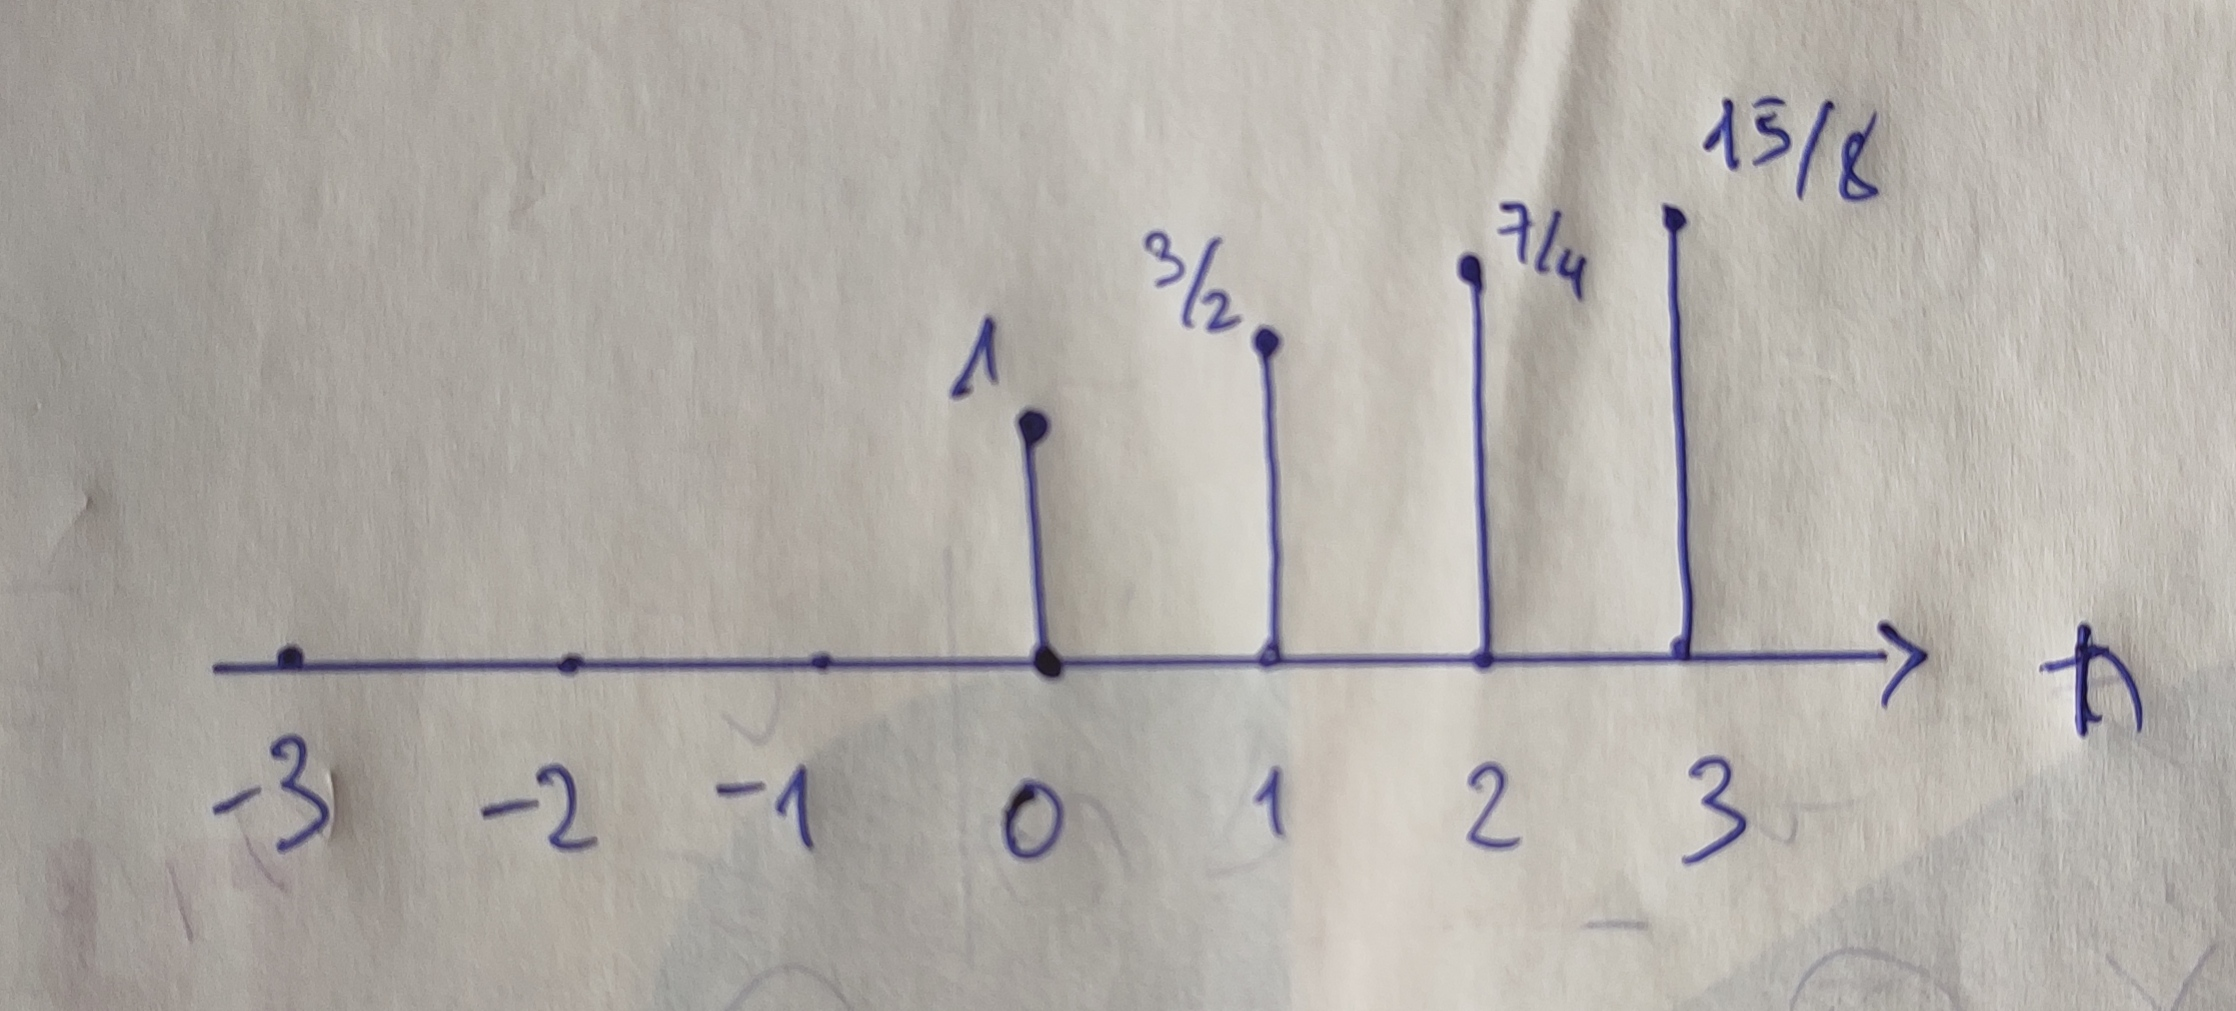
\includegraphics[scale=0.1]{fig/2.3.jpg}
        \end{center}
    \end{figure}

\question Câu 2.7
\begin{parts}
    \part Ta có:
    \begin{equation*}
        x[n] = \delta[n-1]
    \end{equation*}
    \begin{equation*}
        \Rightarrow y_a[n] = \sum_{k = -\infty}^{\infty}{x[k] g[n-2k]} =\sum_{k = -\infty}^{\infty}{\delta[k-1] g[n-2k]} = g[n-2] = u[n-2] - u[n-6]
    \end{equation*}

    \part Tương tự (a):
    \begin{equation*}
        y_b[n] = \sum_{k = -\infty}^{\infty}{x[k] g[n-2k]} =\sum_{k = -\infty}^{\infty}{\delta[k-2] g[n-2k]} = g[n-4] = u[n-4] - u[n-8]
    \end{equation*}

    \part Đầu vào của (b) chính là đầu vào của (a) được dịch sang phải 1 đơn vị. Nếu hệ thống trên là LTI thì đầu ra của (a) dịch phải 1 đơn vị phải bằng đầu ra của câu b. Tuy nhiên có thể thấy:
    \begin{equation*}
        y_a[n-1] = u[n-3] - u[n-7] \neq y_b[n]
    \end{equation*}
    Do đó, hệ thống trên không phải là một hệ thống LTI

    \part Ta có:
    \begin{equation*}
        y_d[n] = \sum_{k = -\infty}^{\infty}{x[k] g[n-2k]} =\sum_{k = 0}^{\infty}{g[n-2k]}
    \end{equation*}
\end{parts}


\question Câu 2.9 \\
    Ta có:
    \begin{equation*}
        h(k) = e^{2k}u(-k+4) + e^{-2k}u(k - 5) = 
        \begin{cases}
            e^{2k}, & k < 4 \\
            e^{-2k}, & k > 5 \\
            0, & 4 < k < 5
        \end{cases}
    \end{equation*}
    Đặt $k = t - \tau$:
    \begin{equation*}
        \Rightarrow h(t-\tau) = 
        \begin{cases}
            e^{2(t-\tau)}, & \tau > t - 4 \\
            e^{-2(t-\tau)}, & \tau < t - 5 \\
            0, & t - 5 < \tau < t - 4
        \end{cases}
    \end{equation*}
    Vậy $ A = t - 5$ và $B = t - 4$


\question Câu 2.13
    \begin{parts}
        %Câu a
        \part Ta có: 
        \begin{equation*}
            \left(\frac{1}{5}\right)^n u[n]-A\left(\frac{1}{5}\right)^{n - 1} u[n - 1] = \delta[n]
        \end{equation*}
        Gán $n = 1$, ta được:
        \begin{equation*}
            \frac{1}{5}-A = 0 \Rightarrow A = \frac{1}{5}
        \end{equation*}

        %Câu b
        \part Từ (a), ta có:
        \begin{equation*}
            \begin{aligned}
            h[n] - \frac{1}{5}h[n-1] & =  \delta[n] \\
            \Rightarrow h[n] * (\delta[n] - \frac{1}{5}\delta[n-1]) & =  \delta[n]\\
            \Rightarrow g[n] & = \delta[n] - \frac{1}{5}\delta[n-1] 
            \end{aligned}
        \end{equation*}
    \end{parts}
\question Câu 2.23

\question Câu 2.28
    \begin{parts}
        \part Ta có: 
        \begin{itemize}
            \item Hệ thống có tính nhân quả do $h[n] = 0, \forall n < 0$
            \item Stable do $\sum_{n=0}^{\infty}{\left(\frac{1}{5}\right)^n} = \frac{5}{4} < \infty$
        \end{itemize}
        \part Ta có:
        \begin{itemize}
            \item Uncausal do $h[n] \neq 0$ với $n < 0$
            \item Stable do $\sum_{n=-2}^{\infty}{\left(0.8\right)^n} = 5 < \infty$
        \end{itemize}
        \part Ta có:
        \begin{itemize}
            \item Uncausal do $h[n] \neq 0$ với $n < 0$
            \item Unstable do $\sum_{n=-\infty}^{0}{\left(\frac{1}{2}\right)^n} = \infty$
        \end{itemize}
        \part Ta có:
        \begin{itemize}
            \item Uncausal do $h[n] \neq 0$ với $n < 0$
            \item Stable do $\sum_{n=-\infty}^{3}{5^n} = \frac{625}{4} < \infty$
        \end{itemize}
        \part Ta có
        \begin{itemize}
            \item Causal do $h[n] = 0, \forall n < 0$
            \item Unstable do hạn tử thứ 2 sẽ $\rightarrow \infty$ khi $n \rightarrow \infty$
        \end{itemize}

        \part Ta có:
        \begin{itemize}
            \item Uncausal do $h[n] \neq 0$ với $n < 0$
            \item Stable do $\sum_{n=-\infty}^{\infty}{h[n]} = \frac{625}{4} < \infty$
        \end{itemize}

        \part Ta có:
        \begin{itemize}
            \item Causal do $h[n] = 0, \forall n < 0$
            \item Stable do $\sum_{n=1}^{\infty}{\frac{n}{3^n}} < \infty$ (Sử dụng tiêu chuẩn Cauchy)
        \end{itemize}
    \end{parts}

\question Câu 2.29
    \begin{parts}
        \part Ta có:
        \begin{itemize}
            \item Causal do $h(t) = 0, \forall t < 0$
            \item Stable do $\int_{2}^{\infty}{e^{-4t}dt} = \frac{e^{-8}}{4} < \infty$
        \end{itemize}

        \part Ta có:
        \begin{itemize}
            \item Uncausal do $h(t) \neq 0, \forall t < 0$
            \item Unstable do $\int_{-\infty}^{3}{e^{-6t}dt} = \infty$
        \end{itemize}

        \part Ta có:
        \begin{itemize}
            \item Uncausal do $h(t) \neq 0, \forall t < 0$
            \item Stable do $\int_{-50}^{\infty}{e^{-2t}dt} = \frac{e^{100}}{2} < \infty$
        \end{itemize}

        \part Ta có:
        \begin{itemize}
            \item Uncausal do $h(t) \neq 0, \forall t < 0$
            \item Stable do $\int_{-\infty}^{-1}{e^{2t}dt} = \frac{e^{-2}}{2} < \infty$
        \end{itemize}

        \part Ta có:
        \begin{itemize}
            \item Uncausal do $h(t) \neq 0, \forall t < 0$
            \item Stable do $\int_{-\infty}^{\infty}{e^{-6|t|}dt} = \frac{1}{3} < \infty$
        \end{itemize}

        \part Ta có:
        \begin{itemize}
            \item Causal do $h(t) = 0, \forall t < 0$
            \item Stable do $\int_{0}^{\infty}{\frac{t}{e^t}dt} = 1 < \infty$
        \end{itemize}

        \part Ta có:
        \begin{itemize}
            \item Causal do $h(t) = 0, \forall t < 0$
            \item Unstable do $\int_{0}^{\infty}{e^{(t-100)/100}dt} = \infty$
        \end{itemize}
    \end{parts}

\question Câu 2.40
    \begin{parts}
        \part Ta có:
        \begin{equation*}
            y(t) = \int_{-\infty}^{t}{e^{-(t - \tau)}x(\tau - 2)d\tau}
        \end{equation*}
        Đặt $\tau' = \tau - 2$, ta có:
        \begin{equation*}
            y(t) = \int_{-\infty}^{t - 2}{e^{-(t - \tau' - 2)}x(\tau')d\tau'} = \left[e^{-(t-2)}u(t-2)\right] * x(t)
        \end{equation*}
        Vậy đáp ứng xung $h(t) = e^{-(t-2)}u(t-2)$
    \end{parts}
\question Câu 2.49

\question Câu 3.1 \\
    Ta có:
    \begin{equation*}
        \begin{aligned}
            x(t) &= a_1e^{j(2\pi/T)t} + a_{-1}e^{-j(2\pi/T)t} + a_3e^{3j(2\pi/T)t} + a_{-3}e^{-3j(2\pi/T)t} \\
            &= 2e^{j(2\pi/T)t} + 2e^{-j(2\pi/T)t} + 4je^{3j(2\pi/T)t} - 4je^{-3j(2\pi/T)t}\\
            &= 4cos(\frac{\pi}{4}t)-8sin(\frac{6\pi}{8}t) \\
            &= 4cos(\frac{\pi}{4}t)+8cos(\frac{6\pi}{8}t + \frac{\pi}{2}) \\
        \end{aligned}
    \end{equation*}

\question Câu 3.2 \\
    Ta có:
    \begin{equation*}
        \begin{aligned}
            x(t) &= a_0 + a_2e^{2j(2\pi/N)n} + a_{-2}e^{-2j(2\pi/N)n} + a_4e^{4j(2\pi/N)n} + a_{-4}e^{-4j(2\pi/N)n} \\
             &= 1 + e^{j\pi/4}e^{2j(2\pi/N)n} + e^{-j\pi/4}e^{-2j(2\pi/N)n} + 2e^{j\pi/3}e^{4j(2\pi/N)n} + 2e^{-j\pi/3}e^{-4j(2\pi/N)n} \\
            &= 1 + 2cos(\frac{4\pi}{5}n+\frac{\pi}{4}) + 4cos(\frac{8\pi}{5}n+\frac{\pi}{3}) \\
            &= 1 + 2sin(\frac{4\pi}{5}n+\frac{3\pi}{4}) + 4sin(\frac{8\pi}{5}n+\frac{5\pi}{6})
        \end{aligned}        
    \end{equation*}

\question Câu 3.3 \\
    Ta có:
    \begin{equation*}
        \begin{aligned}
            x(t) &= 2 + \frac{1}{2}e^{j(2\pi/3)t} + \frac{1}{2}e^{-j(2\pi/3)t} - 2je^{j(5\pi/3)t} + 2je^{-j(5\pi/3)t}
        \end{aligned}
    \end{equation*}
    Từ khai triển trên, ta kết luận chu kì cơ bản $T = 6$
    \begin{equation*}
        \Rightarrow \begin{cases}
            a_0 = 2 \\
            a_2 = a_{-2} = \frac{1}{2} \\
            a_5 = -2j \\
            a_{-5} = 2j
        \end{cases}
    \end{equation*}

\question Câu 3.6
    \begin{parts}
        \part Xét:
        \begin{itemize}
            \item Ta có:
            \begin{equation*}
                a_k = 
                \begin{cases}
                    \left(\frac{1}{2}\right)^k, & 0 \leq k \leq 100 \\
                    0, & otherwise
                \end{cases}
            \end{equation*}
            Do $a_k \neq a^*_{-k}$ nên $x_1(t)$ không phải hàm thực

            \item Tương tự:
            \begin{equation*}
                a_k = 
                \begin{cases}
                    cos(k\pi), & -100 \leq k \leq 100 \\
                    0, & otherwise
                \end{cases}
            \end{equation*}
            Do $a_k = a^*_{-k}$ nên $x_2(t)$ là hàm thực

            \item Tương tự:
            \begin{equation*}
                a_k = 
                \begin{cases}
                    jsin(k\pi/2), & -100 \leq k \leq 100 \\
                    0, & otherwise
                \end{cases}
            \end{equation*}
            Do $a_k = a^*_{-k}$ nên $x_3(t)$ là hàm thực
        \end{itemize}

        \part Ta có, tín hiệu tuần hoàn là tín hiệu chẵn nếu hệ số của dãy Fourier biễu diễn tín hiệu đó là hàm chẵn. Do đó, chỉ có $x_2(t)$ là tín hiệu chẵn
    \end{parts}

\question Câu 3.13 \\
    Do $x(t)$ là hàm thực và là hàm lẻ nên các hệ số $a_k$ có giá trị thuần ảo (vì vậy $a_0 = 0$) và cũng là hàm lẻ. Ta có:
    \begin{equation*}
        \begin{aligned}
            a_k & = \frac{1}{8}\int_0^8{x(t)e^{-j(2\pi/8)kt}dt} \\
           & = \frac{1}{8}\int_0^4{e^{-j(2\pi/8)kt}dt} - \frac{1}{8}\int_4^8{e^{-j(2\pi/8)kt}dt} \\
           & = \frac{1}{j\pi k}\left(1 - e^{-j\pi k}\right) \\
           & = 
           \begin{cases}
               0, & k=2u  \\
               \frac{2}{j\pi k}, & k=2u+1
           \end{cases} u \in \mathbb{Z}
        \end{aligned}
    \end{equation*}
    Ta có:
    \begin{equation*}
        y(t) = \sum_{k = -\infty}^{\infty}{a_k H(jk\omega_0)e^{jk\omega_0t}}
    \end{equation*}
    Với $k = 2u (u \in \mathbb{Z})$, ta có:
    \begin{equation*}
        a_k = 0 \Rightarrow a_k H(jk\omega_0)e^{jk\omega_0t} = 0
    \end{equation*}
    Với $k = 2u+1 (u\in \mathbb{Z})$, ta có:
    \begin{equation*}
        H(jk\omega_0) = H(jk(\pi/4)) = \frac{sin(k\pi)}{k(\pi/4)} = \frac{sin(\pi)}{(2u+1)(\pi/4)} = 0
    \end{equation*}
    Vậy $y(t) = 0$

\question Câu 3.14 \\
    Hệ số Fourier của $x[n]$ là:
    \begin{equation*}
        \begin{aligned}
            a_k &= \frac{1}{4}\sum_{k=0}^3{x[n]e^{-j(2\pi/4)kn}} \\
            &= \frac{1}{4} (\forall k \in \mathbb{Z})
        \end{aligned}
    \end{equation*}
    Ta thu được đầu ra $y[n]$ như sau:
    \begin{equation*}
        \begin{aligned}
            y[n] &= \sum_{k = 0}^3{a_k H(e^{j(2\pi/4)k})e^{jk(2\pi/4)kn}} \\
            &= \sum_{k = 0}^3{\frac{1}{4}H(e^{j(2\pi/4)k})e^{jk(2\pi/4)kn}}
        \end{aligned}
    \end{equation*}
    Theo đề bài, ta có:
    \begin{equation*}
        \begin{aligned}
            y[n] &= cos(\frac{5\pi}{2}n + \frac{\pi}{4}) \\
            &= cos(\frac{\pi}{2}n + \frac{\pi}{4}) \\
            &= \frac{1}{2}e^{j(\frac{\pi}{2}n + \frac{\pi}{4})} + \frac{1}{2}e^{-j(\frac{\pi}{2}n + \frac{\pi}{4})} \\
            &= \frac{1}{2}e^{j(\frac{\pi}{2}n + \frac{\pi}{4})} + \frac{1}{2}e^{j(\frac{3\pi}{2}n - \frac{\pi}{4})} \\
        \end{aligned}
    \end{equation*}
    Vậy:
    \begin{equation*}
        \begin{cases}
            H(e^{j0}) = H(e^{j\pi}) = 0 \\
            H(e^{j\frac{\pi}{2}}) = 2e^{j\frac{\pi}{4}} \\
            H(e^{j\frac{3\pi}{2}}) = 2e^{j\frac{-\pi}{4}} \\
        \end{cases}
    \end{equation*}

\question Câu 3.15 \\
    Ta có:
    \begin{equation*}
        y(t) = \sum_{k = -\infty}^{\infty}{a_kH(jk\omega_0)e^{jk\omega_0t}}
    \end{equation*}
    Với $\omega_0 = \frac{2\pi}{T} = 12$. Lại có:
    \begin{equation*}
        H(jk\omega_0) = 0 \Rightarrow |k\omega_0| > 100 \Rightarrow k>8
    \end{equation*}
    \begin{equation*}
        y(t) = \sum_{k = -\infty}^{8}{a_kH(jk\omega_0)e^{jk\omega_0t}} =\sum_{k = -\infty}^{8}{a_ke^{jk\omega_0t}}
    \end{equation*}
    Theo giả thuyết, ta có:
    \begin{equation*}
        \begin{aligned}
        y(t) &= x(t) \\
        \Leftrightarrow \sum_{k = -\infty}^{8}{a_ke^{jk\omega_0t}} &=\sum_{k = -\infty}^{\infty}{a_ke^{jk\omega_0t}} \\
        \Leftrightarrow \sum_{k = 9}^{\infty}{a_ke^{jk\omega_0t}} &= 0 \\
        \Rightarrow a_k = 0 (k > 8)
        \end{aligned}
    \end{equation*}
    Vậy với $k > 8$ thì $a_k = 0$
\question Câu 3.21
    Ta có:
    \begin{equation*}
        \begin{aligned}
            x(t) &= a_1e^{j(2\pi/T)t} + a_{-1}e^{-j(2\pi/T)t} + a_5e^{5j(2\pi/T)t} + a_{-5}e^{-5j(2\pi/T)t} \\
            &= je^{j(2\pi/T)t} - je^{-j(2\pi/T)t} + 2e^{5j(2\pi/T)t} + 2e^{-5j(2\pi/T)t} \\
            &= -2sin(\frac{\pi}{4}t) + 4cos(\frac{5\pi}{4}t) \\ 
            &= -2cos(\frac{\pi}{4}t - \frac{\pi}{2}) + 4cos(\frac{5\pi}{4}t) \\ 
        \end{aligned}
    \end{equation*}

\question Câu 3.22

\question Câu 3.27
    Ta có:
    \begin{equation*}
        \begin{aligned}
            x[n] &= a_0 + a_2e^{2j(2\pi/N)n} + a_{-2}e^{-2j(2\pi/N)n} + a_4e^{4j(2\pi/N)n} + a_{-4}e^{-4j(2\pi/N)n} \\
            &= 2 + 2e^{j\pi/6}e^{j(4\pi/5)n} + 2e^{-j\pi/6}e^{-j(4\pi/5)n} + e^{j\pi/3}e^{j(8\pi/5)n} + e^{-j\pi/3}e^{-j(8\pi/5)n} \\
            &= 2 + 4cos(\frac{4\pi n}{5}+ \frac{\pi}{6}) + 2cos(\frac{8\pi n}{5}+\frac{\pi}{3}) \\
            &= 2 + 4sin(\frac{4\pi n}{5}+ \frac{2\pi}{3}) + 2sin(\frac{8\pi n}{5}+\frac{5\pi}{6}) \\
        \end{aligned}
    \end{equation*}

\end{questions}

\end{document}